% !TeX root = ../Thesis.tex
\documentclass[../Thesis.tex]{subfiles}
\graphicspath{{\subfix{../images/}}}

\begin{document}

\section{Mid-level Intermediate Representation (MIR)}

An overview of the \acrfull{MIR} is provided in this section.
\acrshort{MIR} was introduced in
\href{https://rust-lang.github.io/rfcs/1211-mir.html}{RFC 1211}
in August 2015.
We will explore its different parts,
how different code fragments are mapped to them,
and the underlying graph structure.

\begin{listing}
    \begin{minted}{Rust}
        fn main() {
            match std::env::args().len() {
                1 => 2,
                3 => 6,
                _ => 0,
            };
        }
    \end{minted}
    \caption{Simple Rust program to explain the MIR components}
    \label{lst:rust-code-example}
\end{listing}

\begin{longlisting}
    \begin{minted}{Rust}
        // WARNING: This output format is intended for human consumers only
        // and is subject to change without notice. Knock yourself out.
        fn main() -> () {
            let mut _0: ();               // return place in scope 0 at src/main.rs:1:11: 1:11
            let mut _1: usize;            // in scope 0 at src/main.rs:2:11: 2:33
            let mut _2: &std::env::Args;  // in scope 0 at src/main.rs:2:11: 2:33
            let _3: std::env::Args;       // in scope 0 at src/main.rs:2:11: 2:27

            bb0: {
                _3 = args() -> bb1;       // scope 0 at src/main.rs:2:11: 2:27
                                          // mir::Constant
                                          // + span: src/main.rs:2:11: 2:25
                                          // + literal: Const { ty: fn() ->
                                          //   Args {args}, val: Value(<ZST>) }
            }

            bb1: {
                _2 = &_3;                 // scope 0 at src/main.rs:2:11: 2:33
                _1 = <Args as ExactSizeIterator>::len(move _2) -> [return: bb2, unwind: bb4];
                                          // scope 0 at src/main.rs:2:11: 2:33
                                          // mir::Constant
                                          // + span: src/main.rs:2:28: 2:31
                                          // + literal: Const { ty: for<'a> fn(&'a Args) ->
                                          //   usize {<Args as ExactSizeIterator>::len},
                                          //   val: Value(<ZST>) }
            }

            bb2: {
                drop(_3) -> bb3;          // scope 0 at src/main.rs:6:6: 6:7
            }

            bb3: {
                return;                   // scope 0 at src/main.rs:7:2: 7:2
            }

            bb4 (cleanup): {
                drop(_3) -> [return: bb5, unwind terminate]; // scope 0 at src/main.rs:6:6: 6:7
            }

            bb5 (cleanup): {
                resume;                   // scope 0 at src/main.rs:1:1: 7:2
            }
        }
    \end{minted}
    \caption{MIR of Listing \ref{lst:rust-code-example}
        compiled using rustc 1.71.0-nightly in debug mode}
    \label{lst:mir-output-debug-example}
\end{longlisting}

Consider the example code listed in Listing \ref{lst:rust-code-example},
the corresponding \acrshort{MIR}\footnote{The comments in the MIR have been slightly modified to improve the output}
is shown in Listing \ref{lst:mir-output-debug-example}.
Notice the explicit warning at the top of the generated output.
It will be omitted in the subsequent listings for simplicity.
Moreover, output depends on the following factors:

\begin{itemize}
    \item The \emph{rustc} version in use,
          alternatively the release channel (stable, beta, or nightly).
    \item The build type: \emph{debug} or \emph{release}.
          By default, the command \texttt{cargo build} generates a \emph{debug} build,
          while \texttt{cargo build --release} produces a \emph{release} build.
\end{itemize}

To illustrate this variability, Listing \ref{lst:mir-output-release-example}
shows the output when compiling the same program in \emph{release} mode.
The distinguishing feature found in \emph{release} builds is
the presence of the \texttt{StorageLive} and \texttt{StorageDead} statements.
On the other hand, \emph{debug} builds generate
shorter and clearer \acrshort{MIR} that is closer to what the user wrote.
For this reason, unless otherwise stated,
the listings in this work contain \acrshort{MIR} generated in \emph{debug} builds.

\begin{longlisting}
    \begin{minted}{Rust}
        // WARNING: This output format is intended for human consumers only
        // and is subject to change without notice. Knock yourself out.
        fn main() -> () {
            let mut _0: ();               // return place in scope 0 at src/main.rs:1:11: 1:11
            let mut _1: usize;            // in scope 0 at src/main.rs:2:11: 2:33
            let mut _2: &std::env::Args;  // in scope 0 at src/main.rs:2:11: 2:33
            let _3: std::env::Args;       // in scope 0 at src/main.rs:2:11: 2:27

            bb0: {
                StorageLive(_1);          // scope 0 at src/main.rs:2:11: 2:33
                StorageLive(_2);          // scope 0 at src/main.rs:2:11: 2:33
                StorageLive(_3);          // scope 0 at src/main.rs:2:11: 2:27
                _3 = args() -> bb1;       // scope 0 at src/main.rs:2:11: 2:27
                                          // mir::Constant
                                          // + span: src/main.rs:2:11: 2:25
                                          // + literal: Const { ty: fn() ->
                                          //   Args {args},
                                          //   val: Value(<ZST>) }
            }

            bb1: {
                _2 = &_3;                 // scope 0 at src/main.rs:2:11: 2:33
                _1 = <Args as ExactSizeIterator>::len(move _2) -> [return: bb2, unwind: bb4];
                                          // scope 0 at src/main.rs:2:11: 2:33
                                          // mir::Constant
                                          // + span: src/main.rs:2:28: 2:31
                                          // + literal: Const { ty: for<'a> fn(&'a Args) ->
                                          //   usize {<Args as ExactSizeIterator>::len},
                                          //   val: Value(<ZST>) }
            }

            bb2: {
                StorageDead(_2);          // scope 0 at src/main.rs:2:32: 2:33
                drop(_3) -> bb3;          // scope 0 at src/main.rs:6:6: 6:7
            }

            bb3: {
                StorageDead(_3);          // scope 0 at src/main.rs:6:6: 6:7
                StorageDead(_1);          // scope 0 at src/main.rs:6:6: 6:7
                return;                   // scope 0 at src/main.rs:7:2: 7:2
            }

            bb4 (cleanup): {
                drop(_3) -> [return: bb5, unwind terminate]; // scope 0 at src/main.rs:6:6: 6:7
            }

            bb5 (cleanup): {
                resume;                   // scope 0 at src/main.rs:1:1: 7:2
            }
        }
    \end{minted}
    \caption{MIR of Listing \ref{lst:rust-code-example}
        compiled using rustc 1.71.0-nightly in release mode}
    \label{lst:mir-output-release-example}
\end{longlisting}

The specific formatting when converting \acrshort{MIR} to a string has changed only slightly over time.
See \cite[Section 3.3]{meyer2020} for an example of older output from mid-2019.

\begin{figure}[!htb]
    \centering
    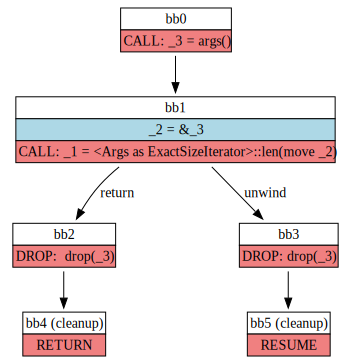
\includegraphics[scale=0.60]{mir-cfg-example.png}
    \caption{The control flow graph representation of the MIR shown in Listing \ref{lst:mir-output-debug-example}}
    \label{fig:mir-cfg-example}
\end{figure}


\end{document}